PD kontrolör
\begin{equation}
    F(s)=k_d s+k_p
\end{equation}
olmak üzere kapalı çevrim transfer fonksiyonu 
\begin{equation}
\begin{split}
    T(s)&=\frac{F(s)G(s)}{1+F(s)G(s)}\\
    &=\frac{(k_d s+k_p)\frac{1}{s^2+s+1}}{1+(k_d s+k_p)\frac{1}{s^2+s+1}}\\
    &=\frac{(k_d s+k_p)}{s^2+(k_d+1)s+(k_p+1)}
\end{split}
\end{equation}
olarak elde edilmektedir. Tasarım için 
\begin{equation}
\begin{split}
    k_d+1&=8\\
    k_p+1&=45.7844
\end{split}
\end{equation}
eşitliğinin çözümü $k_d=7$ ve $k_p=44.7844$ elde edilmektedir. Kapalı çevrim transfer fonksiyonu
\begin{equation}
    T(s)=\frac{7 s + 44.78}{s^2 + 8 s + 45.78}
\end{equation}
olarak hesaplanmaktadır. Basamak yanıtı Şekil~\ref{fig:pd_kontrol} ile gösterilmektedir.
\begin{figure}[!htb]
    \centering
    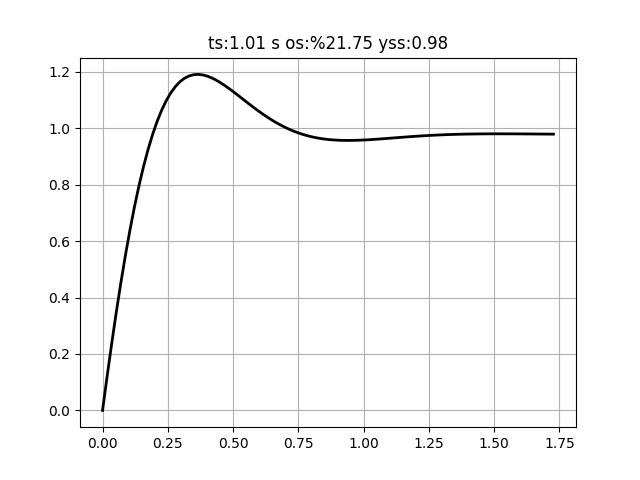
\includegraphics[width=0.75\textwidth]{pd_kontrol}
    \caption{PD kontrolör}
    \label{fig:pd_kontrol}
\end{figure}